


\section{Wat is een PWA}


Het web is een platform waar applicaties kunnen gepubliceerd worden zonder afhankelijk te zijn van een overkoepelend bedrijf of organisatie. Voor een website is er slechts één codebase en de laatste versie is steeds beschikbaar voor de gebruiker. 
Dit allemaal zorgt ervoor dat een webapplicatie iedereen overal kan bereiken en dit op elk mogelijk toestel.

Native applicaties zijn betrouwbaar en bieden een heel goede gebruikerservaring. Ze starten op als een alleenstaande toepassing en ze kunnen uitgebreid gebruik maken van het besturingssysteem: ze kunnen bestanden lezen en schrijven, gebruik maken van usb-connecties en bluetooth, ze hebben toegang tot de contacten en de kalender en nog veel meer. Native applicaties voelen aan alsof ze deel uitmaken van het toestel waarop ze werken.

We kunnen dus stellen dat webapplicaties de bovenhand hebben in bereik maar dat native applicaties de bovenhand hebben als het op functies aankomt.

Een Progressive web application (PWA) is een webapplicatie die gebruik maakt van moderne web API’s om functies aan te bieden die voordien enkel beschikbaar waren voor native applicaties. De bedoeling van PWA’s is om de sterktes van webapplicaties (het bereik) en native applicaties (de functionaliteit) te combineren. 


\autocite{Richard2020}
\autocite{Google2020}



%TODO: alt text bij foto's

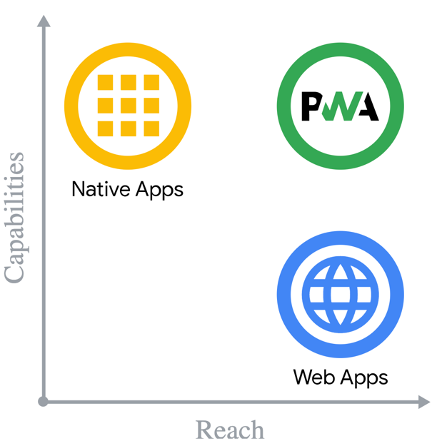
\includegraphics{./img/WatIsEenPwa.png}{voorstelling van wat is een PWA \autocite{Richard2020}}



\subsection{Service workers}

De service worker is een script dat veel functionaliteiten beschikbaar maakt die voordien enkel beschikbaar waren voor native applicaties. In dit hoofdstuk wordt er bekeken welke functionaliteiten de service worker juist beschikbaar maakt en hoe dit gebeurt. 



\subsubsection{Wat is een service worker}

Een service worker is een web worker die tussen het netwerk en de applicatie wordt geplaatst. Dit zorgt ervoor dat de service worker inkomende en uitgaande netwerkverzoeken kan controleren en eventueel manipuleren.
\autocite{Mozilla2020}

Een web worker is een script dat in de achtergrond van een applicatie werkt en die onafhankelijk is van de andere scripts. Web workers hebben dus geen impact op de prestaties van op de webapplicatie die er gebruik van maakt.  Web workers hebben geen toegang tot de DOM van een webapplicatie, ze kunnen de inhoud van een website dus niet rechtstreeks manipuleren.

\autocite{Verdu2015}
\autocite{Hiltunen2018}


Services workers werken dus constant op de achtergrond, maar de manier waarop service workers opgebouwd zijn (zie hoofdstuk service worker lifecycle) heeft geen significante invloed op de batterijduur van een mobiel toestel.

\autocite{Malavolta2016}


\subsubsection{Functionaliteiten die een serivce worker mogelijk maakt}

De service worker werkt onafhankelijk van de applicatie. Dit houdt in dat een service worker wel nog kan werken terwijl de applicatie afgesloten is. Hierdoor zijn volgende functies mogelijk binnen een webapplicatie:


\paragraph{Offline gebruik}
en er is geen internetverbinding, dan zal de service worker de client antwoorden met een boodschap dat er geen internetverbinding is. Zonder een service worker zou de applicatie crashen.

Met service workers kunnen netwerkverzoeken en pagina’s ook gecached worden. Als een pagina geladen wordt, kunnen alle elementen opgeslagen worden op het toestel. Als deze pagina later opnieuw bezocht wordt, hoeft deze niet meer aan de server gevraagd te worden. Hierdoor wordt de applicatie sneller en minder afhankelijk van de netwerkverbinding.
Volgens onderzoek, dat uitgevoerd werd door Google, verlaten 53\% procent van de gebruikers een website als deze niet geladen is binnen 3 seconden. Service workers kunnen dus helpen om het aantal gebruikers op jouw website te verhogen.

\autocite{Google2017}

De twee mechanismes die gebruikt worden om data offline beschikbaar te maken zijn ‘indexedDB’ en de ‘cache API’.
\autocite{Osmani2019}
\autocite{Mozilla2020a}

De cache API wordt gebruikt om data die verkregen werd van netwerkverzoeken op te slaan. Zowel de ‘request’ als de ‘response’ van een netwerkverzoek kunnen in de cache API opgeslagen worden.
\autocite{Scales2019}


IndexedDB is een mechanisme dat gebruikt wordt om lokaal gestructureerde data op te slaan. Het kan vergeleken worden met traditionele relationele databasemanagementsystemen. Er wordt echter geen gebruik gemaakt van kolommen maar van javascript-objecten. 
Een IndexedDb maakt gebruik van indexen. Dit heeft als voordeel dat het uitlezen van data snel kan gebeuren.
\autocite{Mozilla2019}


\paragraph{Notificaties}

Er zijn twee soorten notificaties: lokale notificaties en push notificaties. 
Lokale notificaties worden geactiveerd vanop de applicatie van de gebruiker, er zijn geen externe invloeden die deze notificatie activeren.

Binnen lokale notificaties kunnen we nog het onderscheid maken tussen persistente en niet-persistente notificaties.
Niet-persistente notificaties zijn notificaties die enkel getoond kunnen worden als de applicatie geopend is. Dit type notificaties heeft geen service worker nodig. 
Persistente notificaties zijn notificaties die nog steeds geactiveerd worden vanuit de code op het toestel, maar de applicatie moet niet meer actief zijn. Hier is wel een service worker nodig.

Push notificaties worden niet geactiveerd binnen de applicatie, maar worden geactiveerd door een server.
Om push notificaties te gebruiken, moet er gebruik gemaakt worden van twee webAPI’s: de notifications API en de Push API.

\subparagraph{Notifications API}
Dit is een API die het uiterlijk en het gedrag van een notificatie zal bepalen. Deze API wordt zowel gebruikt voor lokale als voor push notifications.
Om gebruik te maken van deze API moet de gebruiker expliciet toegang geven aan de applicatie.

Een voorbeeld van de code van een notificatie kan er als volgend uitzien



\begin{lstlisting}
function displayNotification() {
  if (Notification.permission == 'granted') {
    navigator.serviceWorker.getRegistration().then(function(reg) {
      var options = {
        body: 'Here is a notification body!',
        icon: 'images/example.png',
        vibrate: [100, 50, 100],
        data: {
          userId: “383209489398274”
        },
        actions: [
          {action: 'explore', title: 'Explore this new world',
            icon: 'images/checkmark.png'},
          {action: 'close', title: 'Close notification',
            icon: 'images/xmark.png'},
        ]
      };
      reg.showNotification('Hello world!', options);
    });
  }
}
\end{lstlisting}


Om een notificatie weer te geven, wordt er een object verwacht waar de inhoud van de melding wordt vastgelegd. Volgende keys kunnen meegegeven worden:


\begin{table}[]
\begin{tabular}{ll}
Body    & De boodschap die in de melding staat.\\
Icon    & Het icoontje dat in de notificatie wordt getoond.\\
Vibrate & Het vibratiepatroon dat de melding zal maken in milliseconden.\\
Data    & Data is een object dat gebruikt kan worden als de gebruiker op de notificatie klikt. Dit object zal dan ontvangen worden in de applicatie. Hier zal vaak het id van de gebruiker teruggevonden worden.\\
Actions & Er kunnen ook acties toegevoegd worden aan de melding. Elk object in deze array zal een knop worden op de melding met een andere functie. Het gedrag van de knoppen wordt bepaald in de applicatie aan de hand van de ‘action’.
\end{tabular}
\caption{tabel: beschrijving notifications API}
\label{tab:notificatie code}
\end{table}

\autocite{GoogleDevelopers2019}
\autocite{Mozilla2019a}



\subparagraph{Push API}

De push API wordt gebruikt door de service worker. Als de server een notificatie verstuurt, wordt deze opgevangen door de push API. Deze push API zal dan gebruik maken van de notifications API om een melding op het toestel van de eindgebruiker te tonen.
\autocite{Mozilla2019b}
\autocite{Gaunt2020}

\paragraph{Achtergrondsynchronisatie }
Een PWA kan gebruik maken van de background sync API om achtergrondsynchronisatie toe te passen.

Achtergrondsynchronisatie kan toegepast worden als er een trage of geen netwerkverbinding is. 

Achtergrondsynchronisatie is het proces waarbij een netwerkverzoek, dat uitgevoerd werd als er geen of een te zwakke internetverbinding was, wordt opgeslagen in de service worker en wordt uitgevoerd als er wel een stabiele internetconnectie is.

Een voorbeeld hiervan is het verzenden van een bericht via een sociaal media platform. Als het bericht verzonden wordt terwijl de gebruiker offline is, zal er geen fout getoond worden maar zal dit bericht verzonden worden vanaf er internet is.

Google Chrome op Android maakt hier gebruik van. Als er een website bezocht wordt als er geen internetverbinding is, krijgt de gebruiker de melding: “Chrome laat je weten wanneer de pagina klaar is”. Vanaf het toestel de pagina heeft kunnen downloaden, krijgt de gebruiker een melding dat de pagina nu bekeken kan worden.



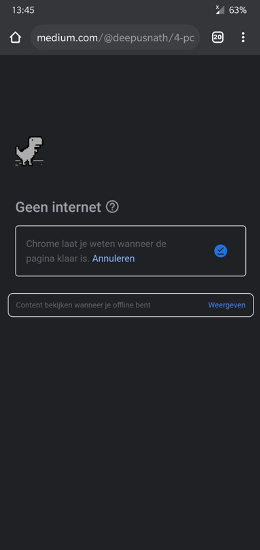
\includegraphics{./img/backSync1.png}{}
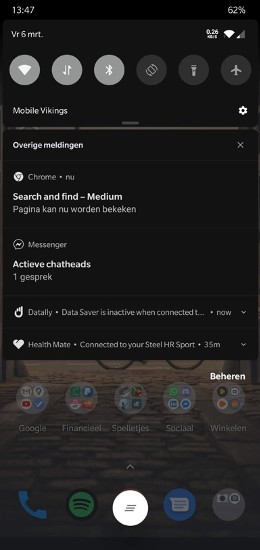
\includegraphics{./img/backSync2.png}{Demonstratie van achtergrond synchronisatie bij Google Chrome op Android}


\subsubsection{Service worker lifecycle }
De levenscyclus van de service worker is onafhankelijk van de levenscyclus van de webapplicatie. Als de webapplicatie gesloten wordt, blijft de service worker gewoon werken.

Om een service worker te installeren moet deze geregistreerd worden in de javascript van de webapplicatie. Dit gebeurt normaal bij het eerst bezoek aan de website van de gebruiker.

\begin{lstlisting}
function displayNotification() {
if ('serviceWorker' in navigator) {
  navigator.serviceWorker.register('/service-worker.js');
}

\end{lstlisting}

Als een service worker wordt geïnstalleerd, worden de opgegeven statische bestanden (foto’s, css-bestanden, javascript-bestanden) gedownload. Als dit slaagt, wordt er naar de activatiefase gegaan, als dit niet slaagt zal dit proces zich herhalen tot het slaagt. 

Tijdens de activatiefase wordt er bekeken welke gecachete gegevens geüpdatet moeten worden en welke niet. De service worker zal de bestanden die het ontvangen heeft van het eerste netwerkverzoek vergelijken met zijn huidig cachegeheugen. Als er verschillen zijn zal dit cachegeheugen aangepast worden.

ls de activatiefase geslaagd is, heeft de service worker controle over de pagina’s die binnen zijn scope vallen. Deze scope moet gedefinieerd worden binnen de service worker.

Nu het oude cachegeheugen up-to-date is, zal de service worker overgaan naar een “rust”-toestand, hierbij wacht de service worker op netwerkverzoeken van bestanden die binnen zijn scope vallen.

Als er een netwerkverzoek wordt verstuurd, zal de service worker deze verzoeken afhandelen. Na een bepaalde tijd zal de service worker terug naar de ‘rust’-modus gaan tot er een nieuw netwerkverzoek is. De service worker gaat naar deze ‘rust’-toestand om zowel cpu-kracht als geheugen te sparen.


\autocite{Gaunt2019}


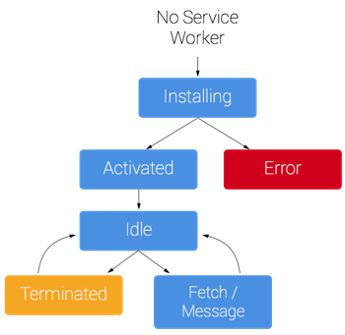
\includegraphics{./img/ServiceWorkerLifeCycle.png}{Schema levenscyclus van een service worker \autocite{Gaunt2019}}




\subsection{A2HS}

Als een applicatie voldoet aan bepaalde criteria, kan deze geïnstalleerd worden op het toestel van de gebruiker. Deze functie is beschikbaar voor verschillende besturingssystemen: Windows, Mac OS, Android, IOS.

Een website moet voldoen aan volgende criteria:

\begin{itemize}
	\item	Nog niet geïnstalleerd zijn
	\item	Een HTTPS-connectie hebben
	\item	Een manifest.json bestand hebben
	\item	Een service worker registreren.
S
\end{itemize}

Als een website aan alle criteria voldoet zal er een beforeinstallprompt event gestart worden. Elke browser gaat hier anders mee om. 


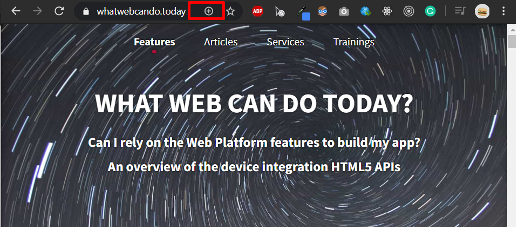
\includegraphics{./img/beforeinstallprompt_windows.png}
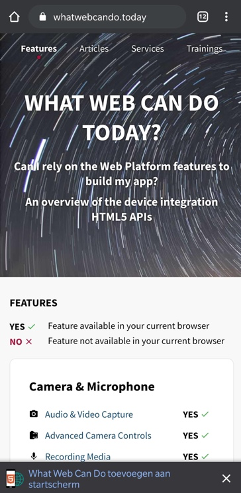
\includegraphics{./img/beforeinstallprompt_android.png}{Gedrag van Google Chrome op desktop en Android.}



